% !TEX root = ../master.tex
\chapter{Implementation and Evaluation}
\label{chap:impl}

%TODO
%similar systems which have a broader scope already papented by otis:
%\autocite{lin2011control}
%\autocite{xang2016trafficlist}
%\section{Volume Estimation in Cabins}
%TODO elipses \autocite[][Chap.~2]{starkosch2010handbook}
%\section{Volume Estimation in Front of Doors}
%\section{Integration into Existing Scheduling Algorithms}
%security considerations?
%other usecases such as door control
%TODO
%\section{Validation}

\section{Visual System}
TODO
\subsection{Implementation with OpenCV and Python}

based on \autocite[][]{xocoatzin2013voxelcarving}

TODO
\subsection{Test Execution}
elevator setup: measurements, camera positions
scenario: empty, single person, 2 persons, 3 persons, only carton, 1+ carton, 2+ carton
TODO
\subsection{Result Evaluation}
general concept feasible
small viewing angle: person out of frame
poor foreground separation by only applying background subtraction
non-correct othorgonal intersection implemented

TODO

\section{Scheduling Algorithm}
TODO
\subsection{Implementation of Simulation}

TODO

The simulation is implemented in the \emph{Rust} programming language.
Rust is a programming language initially developed by Mozilla.
According to its website it is a \enquote{systems programming language that runs blazingly fast, prevents segfaults, and guarantees thread safety} \autocite{rust2018rust}.
It features an expressive static type system and can be used to build applications that take advantage of modern hardware
\autocite[][]{matsakis2014rust}.
The rust compiler targets common platforms and operating and compiles source code to native machine code.
The language is chosen, since the author is proficient in it.

Rust comes with a build tool and package manager named \emph{cargo}. 

TODO describe cargo invocation, describe general programm flow

general program flow:
1. initialize building, lift and general simulation parameters
2. generate 1000 traffic patters, each of one hour, the amount of arrivals of passangers and cargo is described by two poisson distribution,  the traffic items are chosen from the  list of prototypes given
3. for each of the traffic sequences run the simulation with the three differet scheduling strategies. each simulation is given the same parameters and the same traffic pattern
4. collect the results of all the simulations and filter out any rusults whetre any of the three strategies produced invalid results
5. calculate the specified metrics from all the results for each strategy and print them

to run a single simulation with a control strategy:
1. create a new Elevator system state to be altered during the simulation
2. while the current tick of the simulation is smaller than the total ticks of the traffic pattern:
    2.1 ask the control strategy for an action to be performed on the elevator system based on the current state of the elevator system and the current state of the control strategy. also have it return the next control strategy state. The cations can be
    a) move the lift up one floor
    b) move the lift down one floor
    c) open lift doors
    d) close lift doors
    e) load the traffic items from the floor queue into the lift
    f) unload the traffic items from the lift, that need to exit on the current floor
    g) do nothing and idle
    2.2 perform the specified action, thereby updating the state of the lift system
    2.3 advance the current ticks by the amount of time the performed actions took
    2.4 update the metric information about the ride and wait times for each passenger / cargo item
    2.5 copy the traffic times from the traffic pattern to the floor queues, which arrived in the time the last action took
3. correct the metrics by remove ride times of passengers who did not arrive at the destination yet and remove the waiting times of not yet picked up passengers

\begin{figure}
    \centering
    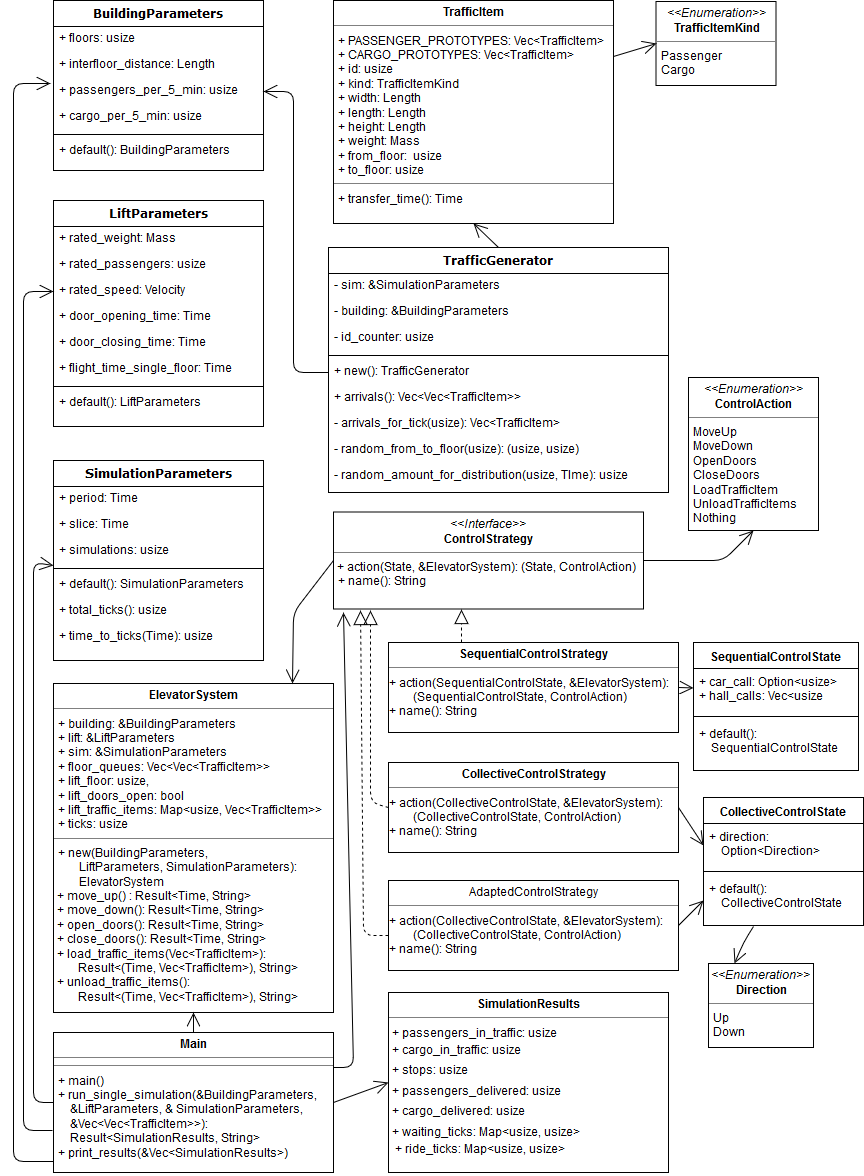
\includegraphics[width=1.0\textwidth, keepaspectratio]{sim_uml_class}
    \caption{Class diagram for simulation programm}
    \label{fig:my_label}
\end{figure}



\subsection{Evaluation of Simulation Results}

TODO

\begingroup
\renewcommand*{\arraystretch}{1.0}
\begin{table}[]
\centering
\begin{tabular}{llrrr}
                                      &     & \begin{minipage}{2cm}\textbf{Sequential Control} \vspace{1em}\end{minipage} & \begin{minipage}{2cm}\textbf{Collective Control} \vspace{1em}\end{minipage} & \begin{minipage}{2cm}\textbf{Adaptive Control} \vspace{1em}\end{minipage}\\ \hline
\multirow{4}{*}{\textbf{Total passengers}}     & \textbf{min}        & 57.00                                                                                                                                             & 57.00                                                                                                                                             & 57.00                                                                                                                                           \\
                                               & \textbf{max}        & 113.00                                                                                                                                            & 113.00                                                                                                                                            & 113.00                                                                                                                                          \\
                                               & \textbf{avg}        & 84.09                                                                                                                                             & 84.09                                                                                                                                             & 84.09                                                                                                                                           \\
                                               & \textbf{$ \sigma $} & 8.97                                                                                                                                              & 8.97                                                                                                                                              & 8.97                                                                                                                                            \\ \hline
\multirow{4}{*}{\textbf{Total cargo}}          & \textbf{min}        & 9.00                                                                                                                                              & 9.00                                                                                                                                              & 9.00                                                                                                                                            \\
                                               & \textbf{max}        & 42.00                                                                                                                                             & 42.00                                                                                                                                             & 42.00                                                                                                                                           \\
                                               & \textbf{avg}        & 24.10                                                                                                                                             & 24.10                                                                                                                                             & 24.10                                                                                                                                           \\
                                               & \textbf{$ \sigma $} & 4.95                                                                                                                                              & 4.95                                                                                                                                              & 4.95                                                                                                                                            \\ \hline
\multirow{4}{*}{\textbf{Stops}}                & \textbf{min}        & 102.00                                                                                                                                            & 93.00                                                                                                                                             & 96.00                                                                                                                                           \\
                                               & \textbf{max}        & 135.00                                                                                                                                            & 158.00                                                                                                                                            & 157.00                                                                                                                                          \\
                                               & \textbf{avg}        & 118.47                                                                                                                                            & 125.75                                                                                                                                            & 129.60                                                                                                                                          \\
                                               & \textbf{$ \sigma $} & 5.22                                                                                                                                              & 10.41                                                                                                                                             & 9.30                                                                                                                                            \\ \hline
\multirow{4}{*}{\textbf{Passengers delivered}} & \textbf{min}        & 37.00                                                                                                                                             & 46.00                                                                                                                                             & 53.00                                                                                                                                           \\
                                               & \textbf{max}        & 65.00                                                                                                                                             & 107.00                                                                                                                                            & 108.00                                                                                                                                          \\
                                               & \textbf{avg}        & 49.32                                                                                                                                             & 78.06                                                                                                                                             & 79.67                                                                                                                                           \\
                                               & \textbf{$ \sigma $} & 4.24                                                                                                                                              & 9.45                                                                                                                                              & 8.75                                                                                                                                            \\ \hline
\multirow{4}{*}{\textbf{Cargo delivered}}      & \textbf{min}        & 3.00                                                                                                                                              & 3.00                                                                                                                                              & 4.00                                                                                                                                            \\
                                               & \textbf{max}        & 23.00                                                                                                                                             & 29.00                                                                                                                                             & 33.00                                                                                                                                           \\
                                               & \textbf{avg}        & 14.13                                                                                                                                             & 14.61                                                                                                                                             & 19.80                                                                                                                                           \\
                                               & \textbf{$ \sigma $} & 3.20                                                                                                                                              & 3.54                                                                                                                                              & 4.38                                                                                                                                            \\ \hline
\multirow{4}{*}{\textbf{Waiting time / s}}     & \textbf{min}        & 1.50                                                                                                                                              & 0.00                                                                                                                                              & 0.00                                                                                                                                            \\
                                               & \textbf{max}        & 2873.50                                                                                                                                           & 202.60                                                                                                                                            & 662.70                                                                                                                                          \\
                                               & \textbf{avg}        & 688.09                                                                                                                                            & 41.25                                                                                                                                             & 53.03                                                                                                                                           \\
                                               & \textbf{$ \sigma $} & 499.11                                                                                                                                            & 32.63                                                                                                                                             & 48.98                                                                                                                                           \\ \hline
\multirow{4}{*}{\textbf{Ride time / s}}        & \textbf{min}        & 13.00                                                                                                                                             & 13.00                                                                                                                                             & 13.00                                                                                                                                           \\
                                               & \textbf{max}        & 64.00                                                                                                                                             & 2180.20                                                                                                                                           & 1809.70                                                                                                                                         \\
                                               & \textbf{avg}        & 29.57                                                                                                                                             & 125.35                                                                                                                                            & 102.29                                                                                                                                          \\
                                               & \textbf{$ \sigma $} & 13.92                                                                                                                                             & 160.37                                                                                                                                            & 130.77                                                                                                                                         
\end{tabular}
\caption{\label{tab:impl:simulationresults} Simulation results for tested scheduling algorithms}
\end{table}
\endgroup

TODO

see table \ref{tab:impl:simulationresults}
key points:

\begin{itemize}
    \item Adaptive control delivers \textbf{more cargo items} on average than sequential control (\texttt{+}40.13~\%) and collective control (\texttt{+}35.52~\%).
    \item Collective control (\texttt{+}58.27~\%) and adaptive control (\texttt{+}61.53~\%) deliver \textbf{more passengers} on average compared to sequential control. 
    \item Sequential control shows a drastically higher mean waiting time then the other two (\texttt{+}1568.09~\%, \texttt{+}1297.55~\%). However a it features a lower average ride time (\texttt{-}76.41~\%, \texttt{-}71.09~\%), which is is only linear dependent on the travel distance.
    \item Adaptive control shows a slightly higher average waiting time (\texttt{+}30.56~\%) but has a lower (\texttt{-}18.40~\%) average ride time, which is less spread (\texttt{-}18.46~\%) compared to collective control.
\end{itemize}

TODO conclusion for efficiency and feasibility



\section{Economic Considerations}
TODO

- possible use cases -> multistory buildings with a elevator that is used by passengers as well as cargo objects, thinkable are (1) hospitals with elevators that are also used by patient beds, (2) multistory warehouses with cargo lifts, (3) office buildings with auxiliary lifts used by janitors with their carts
- possible customers -> Thyssen, Otis, Kone
- cost structure from hardware and software -> hardware necessary: 4 wide angle non-hd cameras per cabin, beefy computer to process the images (one per elevator or per group), cables, electricity, interconnection to group / elevator controller. software necessarry: image processing, connection to group / elevator controller, adapted scheduling software => moderatly priced hardware, real cost is durable and consistent software, many developer hours are needed
- savings possible from improved scheduling: cargo gets priority therefore cargo is delivered faster. having cargo in the cabin can hinder passengers from entering, therefore giving priority can increase overall capacity utilization which increases throughput -> lower energy needs per passenger / cargo
- build costs: visual system can be sold as optional feature for new elevators, or can be sold as upgrade to existing, can be sold at a premium



\section{Privacy Considerations}
Installing a camera system unavoidably raises privacy and security concerns 
for the individuals that are being filmed.
Especially in elevators, which are publicly accessible, there are legal requirements to fulfill.
In Germany the Federal Data Protection Act, \ac{BDSG} \autocite[][]{bmjv2009bdsg}, 
regulates the usage of video surveillance systems.
Public areas may only observed for specified purposes and the presence of a surveillance system must be indicated,
as well as the name and contact of its controller. 
When the data gathered by the system is no longer needed for the specified purpose, it must be deleted 
\autocite[][§~4]{bmjv2009bdsg}.
The European \ac{GDPR} \autocite{eu2016gdpr} describes similar, more broad principles:  
\emph{data transparency, purpose limitation, data minimization, storage limitation and confidentiality}
\autocite{ico2018gdpr}.
Oriented at this principle the following paragraphs provide privacy consideration about the visual system.

The presented visual system has a \emph{limited purpose}, in that it is only used 
to determine whether passengers or cargo items are present in the elevator cabin 
and what volume they take up. 
These information is used to improve the scheduling of the elevator.

In order to keep the usage of video data \emph{transparent},
passengers should be informed about the video system before they enter the cabin.
This could be done by installing a sign, which indicates the presence of the video system, 
clearly states, for what purpose the video data is used for, 
and who is operating the system and can be contacted in case of issues.
The sign should be in front and inside of the elevator, 
so that potential passengers can decide,
if they want to use the lift and be filmed.

Since the system has a limited purpose, 
only data specific to that purpose should be gathered and processed.
The data usage should be \emph{minimized}.
Only as few cameras as possible, but as many as necessary should be installed in the lift.
Areas that are not of interest for the lift system should not be filmed.
Furthermore the resolution of the cameras should be only as high as necessary.
For purpose of detecting the presence, position and outline of a passenger or cargo object 
in the cabin, it is not required to capture fine details.
The DIN EN 62676-4 norm \autocite[][]{din2016surveillance} recommends 
to use a camera resolution, which captures 25 to 62.5 pixel per meter,
for the purpose of detecting or monitoring people.
In addition the kind of processing of the video data should be limited to the extend neccesary for the purpose of the video system. 
For example it is not necessary to perform face detection, or to identify individuals.
However tracking the path of an individual over the course of their journey might be beneficial for the application.

The presented system can operate in real time.
Only the current video frame is needed to determine the presence and volume of passengers and objects.
Therefore the \emph{storage} of the video data can be \emph{limited}.
There is no need to store the video data at all.

In order to keep the video data \emph{confidential}, 
measures must be taken to prevent access by unauthorized parties.
For the purpose of the system, all data processing can be done locally within the elevator system.
The visual system only needs to interact with the elevator controller.
Therefore there is no need to make the data available to the outside, e.g. the internet.
Doing so would open up unnecessary possibilities for misuse of the video system.

\section{Conclusion}
TODO about visual system, simulation, economic, and privacy